% !TEX root=../root.tex

\subsection{Landing Target Vehicle}
As flight tests were conducted in a small indoor environment,
the landing target
vehicle was designed to be small in an attempt to better extend to outdoor
scenarios in which the UAV is to land on larger vehicles such as trucks or boats.
The target vehicle, pictured in~\figref{fig:landing_vehicle}, was manually
driven during the experiments,
roughly following an oval.
% following a rough oval.
% A ground vehicle was assembled as pictured in~\figref{fig:landing_vehicle}
% % with a
% % 6.1 $cm$ ArUco tag serving as the fiducial landing marker.
% % During the experiments, the landing vehicle was
% and manually driven around the
% perimeter of the room during the experiments.

\begin{figure}
  \centering
  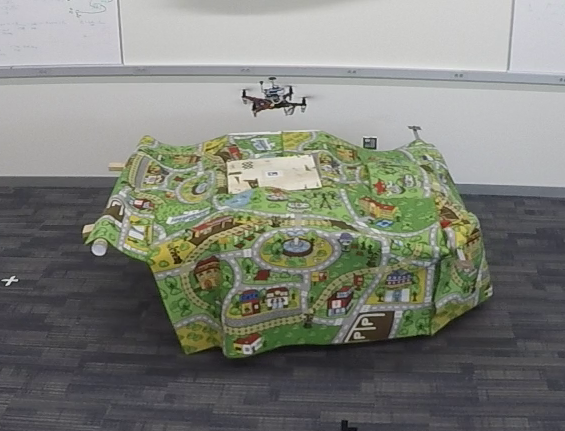
\includegraphics[scale=0.5]{imgs/landing_vehicle.png}
  \caption[UAV Tracking the Target Vehicle During Flight Experiment]{Multirotor
    UAV shown autonomously tracking the landing target
  vehicle.}
  \label{fig:landing_vehicle}
\end{figure}
